\part{Lecture 13: Further Contemporary RL Algorithms}
\title[RL Lecture 13]{Lecture 13: Further Contemporary RL Algorithms}  
\date{}  
\frame{\titlepage} 


%%%%%%%%%%%%%%%%%%%%%%%%%%%%%%%%%%%%%%%%%%%%%%%%%%%%%%%%%%%%%%%%%%
\section{Deep Deterministic Policy Gradient (DDPG)} 
%%%%%%%%%%%%%%%%%%%%%%%%%%%%%%%%%%%%%%%%%%%%%%%%%%%%%%%%%%%%%%%%%%
\begin{frame}
\frametitle{Table of Contents}
\tableofcontents
\end{frame}

%%%%%%%%%%%%%%%%%%%%%%%%%%%%%%%%%%%%%%%%%%%%%%%%%%%%%%%%%%%%%
%% Motivation / General Idea %%
%%%%%%%%%%%%%%%%%%%%%%%%%%%%%%%%%%%%%%%%%%%%%%%%%%%%%%%%%%%%%
\frame{\frametitle{Motivation / General Idea}
\begin{itemize}
	\item The upcoming \hl{deep deterministic policy gradient (DDPG)} algorithm was very much inspired by the successes of DQNs (cf. \algoref{algo:DQN} and landmark \href{https://www.nature.com/articles/nature14236?wm=book_wap_0005}{paper by Mnih et al.}) on discrete action spaces.\pause
	\item However, \hl{DQNs are not directly applicable to (quasi-)continuous action spaces}.\pause
	\item Recall the incremental $Q$-learning  equation using function approximation
	\begin{equation*}
	 \bm{w} \leftarrow \bm{w} + \alpha\left[r+\gamma \max_u \hat{q}(\bm{x}', u, \bm{w}) - \hat{q}(\bm{x}, u, \bm{w})\right]\nabla_{\bm{w}} \hat{q}(\bm{x}, u, \bm{w}).
 \end{equation*}
	\item For every policy inference and updating step we need to find $\max_u \hat{q}(\bm{x}', u, \bm{w})$.\pause 
	\item If $u\in\mathcal{U}\subset\mathbb{Z}$ (i.e., using integer-encoded actions) is a sufficiently small discrete set, that is straightforward by an exhaustive search.\pause
	\item In contrast, if $\bm{u}\in\mathcal{U}\subset\mathbb{R}^m$ is a (quasi-)continuous variable solving $\max_{\bm{u}} \hat{q}(\bm{x}', \bm{u}, \bm{w})$  requires an own \hl{optimization routine} which is computationally expensive if we use nonlinear function approximation. 
\end{itemize}
}

%%%%%%%%%%%%%%%%%%%%%%%%%%%%%%%%%%%%%%%%%%%%%%%%%%%%%%%%%%%%%
%% The Deterministic Policy Trick %%
%%%%%%%%%%%%%%%%%%%%%%%%%%%%%%%%%%%%%%%%%%%%%%%%%%%%%%%%%%%%%
\frame{\frametitle{The Deterministic Policy Trick}
\begin{itemize}
	\item When using a greedy, deterministic policy $\bm{\pi}(\bm{x}, \bm{\theta}) = \bm{\mu}(\bm{x}, \bm{\theta})$ we can utilize it to approximate
	\begin{equation}
		\max_{\bm{u}} \hat{q}(\bm{x}', \bm{u}, \bm{w}) \approx \hat{q}(\bm{x}', \bm{\mu}(\bm{x}, \bm{\theta}), \bm{w}).
	\end{equation}
	\item Hence, we can obtain explicit $Q$-learning targets for continuous actions when using a deterministic policy.\pause 
	\item For improving the policy we reuse the deterministic policy gradient theorem in an off-policy fashion
	\begin{equation}
	\nabla_{\bm{\theta}} J(\bm{\theta}) = \El{\nabla_{\bm{\theta}} \bm{\mu}(\bm{X},\bm{\theta}) \nabla_{\bm{u}} q(\bm{X},\bm{U})\left|\bm{U}=\bm{\mu}(\bm{X}, \bm{\theta})\right.}{b}
\end{equation}
given a behavior policy $b(\bm{u}|\bm{x})$.
\end{itemize}
}

%%%%%%%%%%%%%%%%%%%%%%%%%%%%%%%%%%%%%%%%%%%%%%%%%%%%%%%%%%%%%
%% DDPG $\approx$ DQN + DPG %%
%%%%%%%%%%%%%%%%%%%%%%%%%%%%%%%%%%%%%%%%%%%%%%%%%%%%%%%%%%%%%
\frame{\frametitle{DDPG $\approx$ DQN + DPG}
\begin{itemize}
	\item Hence, we can consider the DDPG approach as a combination of DQN + DPG rendering it an \hl{actor-critic off-policy approach for continuous state and action spaces}.\pause
	\item Similarly to DQN we will introduce \hl{several 'tweaks'} to stabilize and improve the DDPG learning process.\pause	
\end{itemize}
\vspace{0.25cm}
\hl{Tweak \#1}: experience replay buffer
\begin{itemize}
	\item We store $\left\langle \bm{x}, \bm{u}, r, \bm{x}'\right\rangle$ in $\bm{\mathcal{D}}$ after each transition step.\pause
	\item The replay buffer $\bm{\mathcal{D}}$ is of limited capacity, i.e., it discards the oldest data sample when updating once it is full (ring memory).\pause
	\item This allows us to improve the $Q$-learning critic minimizing the mean-squared Bellman error (MSBE):
	\begin{equation}
	\label{eq:MSBE_DDPG}
		\mathcal{L}(\bm{w}) = \left[\left(r+ \gamma q(\bm{x}',\bm{\mu}(\bm{x}',\bm{\theta}),\bm{w})\right) - q(\bm{x},\bm{u},\bm{w}) \right]^2_{\bm{\mathcal{D}}} .
	\end{equation}
\end{itemize}
}

%%%%%%%%%%%%%%%%%%%%%%%%%%%%%%%%%%%%%%%%%%%%%%%%%%%%%%%%%%%%%
%% Additional DDPG Tweaks (1) %%
%%%%%%%%%%%%%%%%%%%%%%%%%%%%%%%%%%%%%%%%%%%%%%%%%%%%%%%%%%%%%
\frame{\frametitle{Additional DDPG Tweaks (1)}
\hl{Tweak \#2}: target networks
\begin{itemize}
	\item Similar to DQN we introduce a (delayed) target network to estimate the $Q$-learning target $$r+ \gamma q(\bm{x}',\bm{\mu}(\bm{x}',\bm{\theta}),\bm{w})$$ since it depends on the same parameters $\bm{w}$ which we want to update.\pause
	\item Hence, the target network's purpose it to mimic the generation of i.i.d. data as the ground truth to minimize \eqref{eq:MSBE_DDPG}.\pause
	\item Since the policy parameters $\bm{\theta}$ are also part of the target calculation it turns out that an additional policy target network is also beneficial to stabilize the $Q$-learning.\pause
	\item In contrast to the classical DQN implementation, the original DDPG algorithm does not perform periodically hard target network updates but continuous ones using a low-pass filter characteristic
	\begin{equation}
		\bm{w}^{-} \leftarrow (1-\tau)\bm{w}^{-}+\tau\bm{w}, \quad \bm{\theta}^{-} \leftarrow (1-\tau)\bm{\theta}^{-}+\tau\bm{\theta}
	\end{equation}
	with $\tau$ representing the equivalent filter constant (hyperparameter).
\end{itemize}
}

%%%%%%%%%%%%%%%%%%%%%%%%%%%%%%%%%%%%%%%%%%%%%%%%%%%%%%%%%%%%%
%% Additional DDPG Tweaks (2) %%
%%%%%%%%%%%%%%%%%%%%%%%%%%%%%%%%%%%%%%%%%%%%%%%%%%%%%%%%%%%%%
\frame{\frametitle{Additional DDPG Tweaks (2)}
\hl{Tweak \#3}: mini-batch sampling
\begin{itemize}
	\item Given a sufficiently filled memory $\bm{\mathcal{D}}$ and the target networks parametrized by $\bm{w}^{-}$ and $\bm{\theta}^{-}$ we draw uniformly distributed mini-batch samples $\bm{\mathcal{D}}_b$ from $\bm{\mathcal{D}}$.\pause
	\item The actual $Q$-learning is then based on the loss
		\begin{equation}
		\label{eq:Loss_DDPG}
				\mathcal{L}(\bm{w}) = \left[\left(r+ \gamma q(\bm{x}',\bm{\mu}(\bm{x}',\bm{\theta}^{-}),\bm{w}^{-})\right) - q(\bm{x},\bm{u},\bm{w}) \right]^2_{\bm{\mathcal{D}}_b} \, .
	\end{equation}
\end{itemize}\pause
\hl{Tweak \#4}: batch normalization
\begin{itemize}
	\item Minimizing \eqref{eq:Loss_DDPG} is a supervised learning step within the DDPG.\pause
	\item The \href{https://arxiv.org/abs/1509.02971}{original DDPG paper by Lillicrap et al.} back in 2015/16 suggested to use batch normalization, i.e., re-centering and re-scaling the inputs of each layer in an ANN.\pause
	\item This idea of batch normalization was presented at that time shortly before by Ioffe and Szegedy (cf. \href{http://proceedings.mlr.press/v37/ioffe15.html}{original paper}).\pause
	\item Today's perspective: stick to the current state-of-the-art supervised ML algorithms for top-class $Q$-learning stability and speed (which are normally well-covered in popular supervised ML toolboxes). 
\end{itemize}
}

%%%%%%%%%%%%%%%%%%%%%%%%%%%%%%%%%%%%%%%%%%%%%%%%%%%%%%%%%%%%%
%% Additional DDPG Tweaks (3) %%
%%%%%%%%%%%%%%%%%%%%%%%%%%%%%%%%%%%%%%%%%%%%%%%%%%%%%%%%%%%%%
\frame{\frametitle{Additional DDPG Tweaks (3)}
\setcounter{footnote}{0}
\hl{Tweak \#5}: exploration
\begin{itemize}
	\item Since our policy is deterministic we require an exploratory behavior policy.\pause
	\item Similar to DPG the standard approach is to add noise to the greedy actions, e.g., again from an Ornstein-Uhlenbeck (OU) process
		\begin{equation*}
			\bm{u}_k\sim\bm{b}(\bm{u}|\bm{x}_k)=\bm{\mu}(\bm{x}_k,\bm{\theta}_k)+\bm{\nu}_{k},\quad \bm{\nu}_{k}= \lambda \bm{\nu}_{k-1}+ \sigma \bm{\epsilon}_{k-1}.
		\end{equation*}\pause
		\item One might also add a schedule for $\lambda$ and $\sigma$ along the training procedure, e.g., starting with significant noise levels (increased exploration) while reducing it over time (focusing exploitation)\footnote{Please note that this 'lambda' is not related to TD($\lambda$), Sarsa($\lambda$), etc. Here, it is representing the stiffness of the OU noise process.}.\pause  
	\item However, many other behavior policies are possible, e.g., using model or expert-based guidance.
\end{itemize}
}

%%%%%%%%%%%%%%%%%%%%%%%%%%%%%%%%%%%%%%%%%%%%%%%%%%%%%%%%%%%%%
%% Summary of DQN Working Principle  (2)%%
%%%%%%%%%%%%%%%%%%%%%%%%%%%%%%%%%%%%%%%%%%%%%%%%%%%%%%%%%%%%%
\frame{\frametitle{Visual Summary of DDPG Working Principle}
\begin{figure}
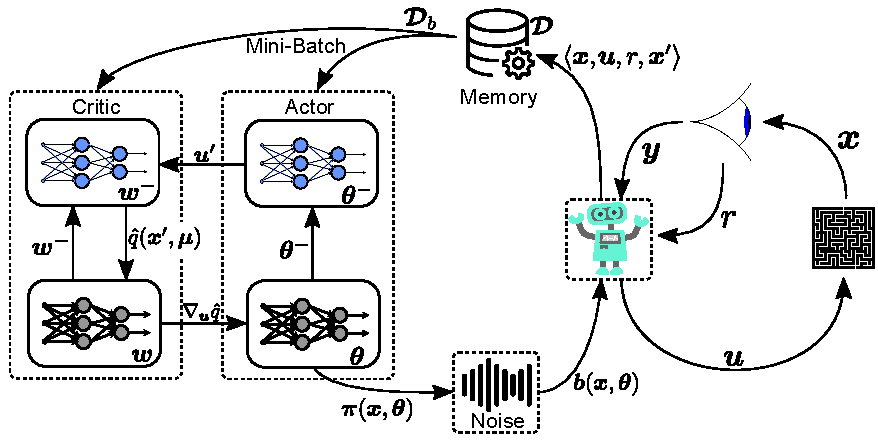
\includegraphics[height=5.75cm]{fig/lec13/DDPG.pdf}
\caption{DDPG structure from a bird's-eye perspective (derivative work of \figref{fig:RL_Wiki} and \href{https://commons.wikimedia.org/wiki/File:Multi-Layer_Neural_Network-Vector.svg?uselang=de}{wikipedia.org}, \href{https://creativecommons.org/publicdomain/zero/1.0/deed.en}{CC0 1.0})}
\label{fig:DDPG}
\end{figure}
}	

%%%%%%%%%%%%%%%%%%%%%%%%%%%%%%%%%%%%%%%%%%%%%%%%%%%%%%%%%%%%%
%% Algorithmic Implementation: DDPG %%
%%%%%%%%%%%%%%%%%%%%%%%%%%%%%%%%%%%%%%%%%%%%%%%%%%%%%%%%%%%%%
\frame{\frametitle{Algo. Implementation: DDPG}
\setlength{\algomargin}{0.5em}
\begin{algorithm}[H]
\small
\SetKwInput{Input}{input} 
\SetKwInput{Output}{output}
\SetKwInput{Init}{init}
\SetKwInput{Param}{parameter}
\Input{diff. det. policy fct. $\bm{\mu}(\bm{x},\bm{\theta})$ and action-value fct. $\hat{q}(\bm{x},\bm{u},\bm{w})$}
\Param{step sizes and filter constant $\{\alpha_{w}, \alpha_{\theta}, \tau\}\in\left\{\mathbb{R}|0<\alpha, \tau<1\right\}$}
\Init{weights $\bm{w}=\bm{w}^{-}\in\mathbb{R}^{\zeta}$ and $\bm{\theta}=\bm{\theta}^{-}\in\mathbb{R}^d$ arbitrarily, memory $\bm{\mathcal{D}}$}\pause
 \For{$j=1,2,\ldots,$ episodes}{
		initialize $\bm{x}_0$\; 
		\For{$k=0,1,\ldots, T-1$ time steps}{
			$\bm{u}_k \leftarrow$ apply from $\bm{\mu}(\bm{x}_k, \bm{\theta})$ w/wo noise or from behavior policy\;
			observe $\bm{x}_{k+1}$ and $r_{k+1}$\;
			store tuple $\left\langle \bm{x}_k, \bm{u}_k, r_{k+1}, \bm{x}_{k+1}\right\rangle$ in $\bm{\mathcal{D}}$\;\pause
			sample mini-batch $\bm{\mathcal{D}}_b$ from $\bm{\mathcal{D}}$ (after initial memory warmup)\;
			\For(calculate $Q$-targets){$i=1,\ldots,b$ samples}{
				\lIf{$\bm{x}_{i+1}$ is terminal}{$y_i=r_{i+1}$}
				\lElse{$y_i= r_{i+1}+ \gamma \hat{q}(\bm{x}_{i+1},\bm{\mu}(\bm{x}_{i+1},\bm{\theta}^{-}),\bm{w}^{-})$}
			}\pause
			fit $\bm{w}$ on loss $\mathcal{L}(\bm{w})=[y - \hat{q}(\bm{x}, \bm{u}, \bm{w})]^2_{\bm{\mathcal{D}}_b}$ with step size $\alpha_{w}$\;\pause
			$\bm{\theta} \leftarrow \bm{\theta} + \alpha_{\theta} [\nabla_{\bm{\theta}}\bm{\mu}(\bm{x},\bm{\theta})\nabla_{\bm{u}}\hat{q}(\bm{x}, \bm{u}, \bm{w})\vert_{\bm{u}=\bm{\mu}_{\bm{\theta}}(\bm{x})}]_{\bm{\mathcal{D}}_b}$\;\pause 
			Update target net. $\bm{w}^{-} \leftarrow (1-\tau)\bm{w}^{-}+\tau\bm{w}, \,\, \bm{\theta}^{-} \leftarrow (1-\tau)\bm{\theta}^{-}+\tau\bm{\theta}$\;
		}
	}
\caption{Deep deterministic policy gradient (output: parameter vectors $\bm{\theta}^*$ for $\bm{\mu}^*(\bm{x},\bm{\theta}^*)$) and $\bm{w}^*$ for $\hat{q}^*(\bm{x}, \bm{u}, \bm{w}^*))$}
\label{algo:DDPG}
\end{algorithm}
}

%%%%%%%%%%%%%%%%%%%%%%%%%%%%%%%%%%%%%%%%%%%%%%%%%%%%%%%%%%%%%%%%%%
\section{Twin Delayed Deep Deterministic Policy Gradient (TD3)} 
%%%%%%%%%%%%%%%%%%%%%%%%%%%%%%%%%%%%%%%%%%%%%%%%%%%%%%%%%%%%%%%%%%
\begin{frame}
\frametitle{Table of Contents}
\tableofcontents[currentsection]
\end{frame}

%%%%%%%%%%%%%%%%%%%%%%%%%%%%%%%%%%%%%%%%%%%%%%%%%%%%%%%%%%%%%
%% Overestimation Bias %%
%%%%%%%%%%%%%%%%%%%%%%%%%%%%%%%%%%%%%%%%%%%%%%%%%%%%%%%%%%%%%
\frame{\frametitle{Overestimation Bias}
\begin{itemize}
	\item For $Q$-learning in the tabular case we have already discussed the \hl{maximization bias} (cf. \figref{Double_Learning_Example}) issue.\pause
	\item Recap: Due to the greedy policy targets, $\hat{q}$ was overestimated when calculated using sampled values of stochastic MDPs.\pause
	\item Additional problem when applying function approximation: the estimator itself introduces additional variance during the learning process which represents another source of the maximization bias problem.\pause
\end{itemize}
\begin{block}{}
This issue is already known in the DQN context (cf. \algoref{algo:DQN}). Similar to the tabular case, \hl{double DQN} introduces a second $Q$-network counteracting the overestimation issue (cf. \href{https://arxiv.org/pdf/1509.06461.pdf}{paper by van Hasselt et al.}).
\end{block}\pause
However, we did not address this possible problem in an actor-critic context using function approximation (e.g., DDPG). 
}

%%%%%%%%%%%%%%%%%%%%%%%%%%%%%%%%%%%%%%%%%%%%%%%%%%%%%%%%%%%%%
%% Overestimation Bias in Actor-Critic Approaches (1) %%
%%%%%%%%%%%%%%%%%%%%%%%%%%%%%%%%%%%%%%%%%%%%%%%%%%%%%%%%%%%%%
\frame{\frametitle{Overestimation Bias in Actor-Critic Approaches (1)}
\begin{itemize}
	\item It turns out that the overestimation bias is also an issue for actor-critic methods as shown next \footnote[1]{Source: S. Fujimoto et al., \textit{Addressing Function Approximation Error in Actor-Critic Methods}, \href{https://arxiv.org/abs/1802.09477}{https://arxiv.org/abs/1802.09477}, 2018}.\pause
	\item Consider an actor-critic policy with the current policy parameters $\bm{\theta}$.\pause
	\item Let $\tilde{\bm{\theta}}$ define the parameters from the actor update induced by the maximization of the approximate critic $\hat{q}_{\bm{w}}(\bm{x}, \bm{u})$. \pause
	\item Let $\bm{\theta}^*$ be the parameters from the hypothetical actor update w.r.t. the true underlying value function $q^{\bm{\pi}}(\bm{x}, \bm{u})$.\pause
	\item Then, we perform the policy update
	\begin{equation}
\begin{aligned}
\tilde{\bm{\theta}} &= \bm{\theta} + \frac{\alpha}{Z_1} \El{\nabla_{\bm{\theta}} \pi_{\bm{\theta}}(\bm{X}) \nabla_{\bm{u}} \hat{q}_{\bm{w}}(\bm{X},\bm{U})\left|\bm{U}=\bm{\pi}_{\bm{\theta}}(\bm{X})\right.}{\pi},\\
\bm{\theta}^* &= \bm{\theta} + \frac{\alpha}{Z_2} \El{\nabla_{\bm{\theta}} \pi_{\bm{\theta}}(\bm{X}) \nabla_{\bm{u}} q^{\bm{\pi}}(\bm{X},\bm{U})\left|\bm{U}=\bm{\pi}_{\bm{\theta}}(\bm{X})\right.}{\pi},
\end{aligned}
\end{equation} 
where $Z_1$ and $Z_2$ normalize the gradient such that $Z^{-1}||\El{\cdot}{}|| = 1$.
\end{itemize}	
}

%%%%%%%%%%%%%%%%%%%%%%%%%%%%%%%%%%%%%%%%%%%%%%%%%%%%%%%%%%%%%
%% Overestimation Bias in Actor-Critic Approaches (2) %%
%%%%%%%%%%%%%%%%%%%%%%%%%%%%%%%%%%%%%%%%%%%%%%%%%%%%%%%%%%%%%
\frame{\frametitle{Overestimation Bias in Actor-Critic Approaches (2)}
\begin{itemize}
	\item Lets denote $\tilde{\bm{\pi}}$ and $\bm{\pi}^*$ as the policies with updated parameters $\tilde{\bm{\theta}}$ and $\bm{\theta}^*$ respectively.\pause
	\item As the gradient direction is a local maximizer, there exists $\epsilon_1$ sufficiently small such that if $\alpha \leq \epsilon_1$ then the \emph{approximate} value of $\tilde{\bm{\pi}}$ will be bounded below by the \emph{approximate} value of $\bm{\pi}^*$:
\begin{equation} \label{eq:approx_q_TD3}
\E{\hat{q}_{\bm{w}}(\bm{X}, \tilde{\bm{\pi}}(\bm{X}))} \geq \E{\hat{q}_{\bm{w}}(\bm{X}, \bm{\pi}^*(\bm{X}))}.
\end{equation}\pause
\item Conversely, there exists $\epsilon_2$ sufficiently small such that if $\alpha \leq \epsilon_2$ then the \emph{true} value of $\tilde{\bm{\pi}}$ will be bounded above by the \emph{true} value of $\bm{\pi}^*$:
\begin{equation} \label{eq:true_q_TD3}
\E{q^{\bm{\pi}}(\bm{X}, \bm{\pi}^*(\bm{X}))} \geq \E{q^{\bm{\pi}}(\bm{X}, \tilde{\bm{\pi}}(\bm{X}))}.
\end{equation}\pause
\item In other words: if the approximate and true critics differ from each other, the according policy gradient updates cannot lead to better policy updates of the respective other framework.  
\end{itemize}	
}

%%%%%%%%%%%%%%%%%%%%%%%%%%%%%%%%%%%%%%%%%%%%%%%%%%%%%%%%%%%%%
%% Overestimation Bias in Actor-Critic Approaches (3) %%
%%%%%%%%%%%%%%%%%%%%%%%%%%%%%%%%%%%%%%%%%%%%%%%%%%%%%%%%%%%%%
\frame{\frametitle{Overestimation Bias in Actor-Critic Approaches (3)}
\begin{itemize}
	\item If the expected, estimated action value will be at least as large as the \textit{true} action value w.r.t. $\bm{\theta}^*$
	\begin{equation}
  \E{\hat{q}_{\bm{w}}(\bm{X}, \bm{\pi}^*(\bm{X}))} \geq \E{q^{\bm{\pi}}(\bm{X}, \bm{\pi}^*(\bm{X}))}, 
\end{equation}\pause
then \eqref{eq:approx_q_TD3} and \eqref{eq:true_q_TD3} imply 
	\begin{equation}
  \E{\hat{q}_{\bm{w}}(\bm{X}, \tilde{\bm{\pi}}(\bm{X}))} \geq \E{q^{\bm{\pi}}(\bm{X}, \tilde{\bm{\pi}}(\bm{X}))}
\end{equation}
	with a sufficiently small $\alpha<\min\{\epsilon_1, \epsilon_2\}$.\pause
	\item Hence, the \hl{maximization bias is also present in actor-critic} updates.\pause
	\item It can add up over several estimation updates and, therefore, may lead to suboptimal policy updates.\pause
	\item A proof for unnormalized gradients can be also found in S. Fujimoto et al., \textit{Addressing Function Approximation Error in Actor-Critic Methods}, 2018.
\end{itemize}	
}

%%%%%%%%%%%%%%%%%%%%%%%%%%%%%%%%%%%%%%%%%%%%%%%%%%%%%%%%%%%%%
%% Overestimation Example for DDPG%%
%%%%%%%%%%%%%%%%%%%%%%%%%%%%%%%%%%%%%%%%%%%%%%%%%%%%%%%%%%%%%
\frame{\frametitle{Overestimation Example for DDPG}
\vspace{0.75cm}
\begin{figure}
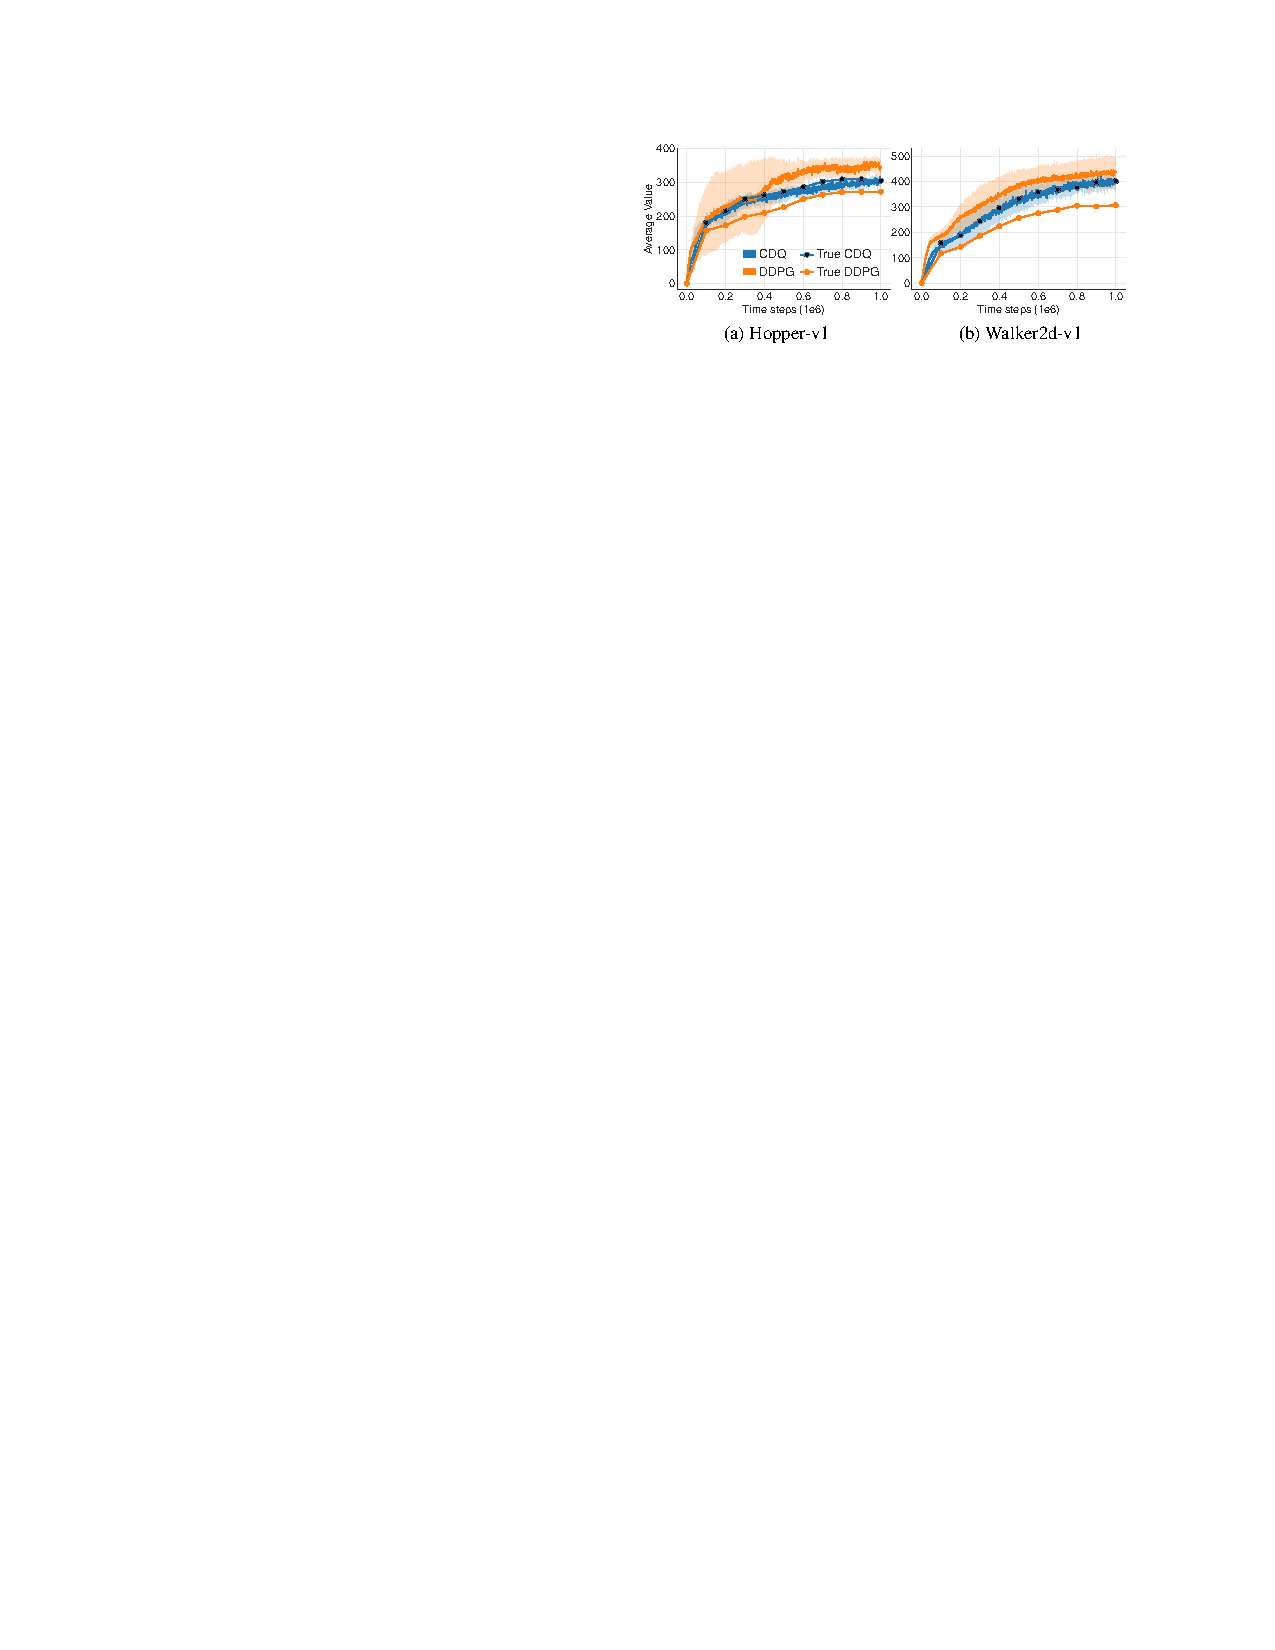
\includegraphics[height=4cm]{fig/lec13/DDPG_Overestimation.pdf}
\caption{Comparison of true and estimated values averaged over 10000 states in two robotic examples from \href{https://gym.openai.com/envs/\#mujoco}{OpenAI Gym}. Estimated values originate from the approximate DDPG critic while the true values are based on the average discounted return over 1000 episodes following the current policy, starting from states sampled from the replay buffer (source: S. Fujimoto et al., \textit{Addressing Function Approximation Error in Actor-Critic Methods}, 2018.}
\label{fig:DDPG_Overestimation}
\end{figure}
}	

%%%%%%%%%%%%%%%%%%%%%%%%%%%%%%%%%%%%%%%%%%%%%%%%%%%%%%%%%%%%%
%% Overestimation Example for DDPG%%
%%%%%%%%%%%%%%%%%%%%%%%%%%%%%%%%%%%%%%%%%%%%%%%%%%%%%%%%%%%%%
\frame{\frametitle{Increased Variance due to Accumulating TD Errors}
\begin{itemize}
	\item Using function approximation, the \hl{Bellman equation is never exactly satisfied} leaving room for some amount of \hl{residual TD-error} $\tilde{\delta}(\bm{x}, \bm{u})$:
	\begin{equation}
		\hat{q}_{\bm{w}}(\bm{x}, \bm{u}) = r + \gamma \El{\hat{q}_{\bm{w}}(\bm{X}', \bm{U}')|\bm{X}'=\bm{x}', \bm{U}'=\bm{u}'}{\pi} - \tilde{\delta}(\bm{x}, \bm{u}).
	\end{equation}\pause
	\item Although this error might be considered small per update step, it may accumulate over future steps if biased:
	\begin{align}
		\hat{q}_{\bm{w}}(\bm{x}, \bm{u}) =\El{\sum_{k=0}^\infty\gamma^{k}\left(R_k-\tilde{\delta}_{k}(\bm{X}, \bm{U})\right)\left|\vphantom{\sum_{k=0}^\infty}\bm{X}=\bm{x}, \bm{U}=\bm{u}\right.}{\pi}.
	\end{align}\pause
	\item Observation: the \hl{variance of $\hat{q}$ will be proportional to the variance of future reward and residual TD-errors}.\pause
	\item If $\gamma$ is large, the estimation variance might increase significantly.\pause
	\item Mini-batch sampling will contribute to this variance issue. 
\end{itemize}
}	

%%%%%%%%%%%%%%%%%%%%%%%%%%%%%%%%%%%%%%%%%%%%%%%%%%%%%%%%%%%%%
%% TD3 Extensions and Modifications (1) %%
%%%%%%%%%%%%%%%%%%%%%%%%%%%%%%%%%%%%%%%%%%%%%%%%%%%%%%%%%%%%%
\frame{\frametitle{TD3 Extensions and Modifications (1)}
\begin{block}{}
	 In order to reduce both the maximization bias and the learning variance, TD3 introduces mainly three measures on top of the DDPG algorithm. Hence, \hl{TD3 is a direct successor of DDPG}. 
\end{block}\pause
\hl{Measure \#1}: clipped double $Q$-learning for actor-critic
\begin{itemize}
	\item Following double $Q$-learning, a pair of critics $\{\hat{q}_{\bm{w}_1}, \hat{q}_{\bm{w}_2}\}$ is introduced.\pause
	\item In contrast, the clipped target (with target networks $\{\bm{w}^{-}_1, \bm{w}^{-}_2\}$)
	\begin{equation}
	\label{eq:Q_clipping_TD3}
		y = r + \gamma \min_{i=1,2}\hat{q}_{\bm{w}^{-}_i}(\bm{x}', \bm{u}')
	\end{equation}
	provides an upper-bound on the estimated action value.\pause
	\item May introduce some underestimation, which is considered less critical than overestimation, since the value of underestimated actions will not be explicitly propagated through the policy update. \pause
	\item The $\min$ operator will also (indirectly) favor actions leading to values with estimation errors of lower variance. 
\end{itemize}
}	

%%%%%%%%%%%%%%%%%%%%%%%%%%%%%%%%%%%%%%%%%%%%%%%%%%%%%%%%%%%%%
%% TD3 Extensions and Modifications (2) %%
%%%%%%%%%%%%%%%%%%%%%%%%%%%%%%%%%%%%%%%%%%%%%%%%%%%%%%%%%%%%%
\frame{\frametitle{TD3 Extensions and Modifications (2)}
\hl{Measure \#2}: target policy smoothing regularization
\begin{itemize}
	\item Background: deterministic policies $\bm{\mu}$ tend to overfit to narrow peaks in the action-value estimate.\pause
	\item Counteraction: fit the action value of a small area around the target action (i.e., smoothing $\hat{q}$ in the action space):
	\begin{equation}
		y = r + \gamma \hat{q}_{\bm{w}^{-}}(\bm{x}', \bm{\mu}_{\bm{\theta}^{-}}(\bm{x}')+\bm{\epsilon}).
	\end{equation}\pause
	\item Here, $\bm{\epsilon}\sim\mathrm{clip}\left(\mathcal{N}(\bm{0},\bm{\Sigma}), -\bm{c},\bm{c}\right)$ is a mean-free, Gaussian noise with covariance $\bm{\Sigma}$, which is clipped at $\pm \bm{c}$ while $\bm{\theta}^{-}$ are the policy target network parameters.\pause
	\item To satisfy possible action constraints (denoted by upper and lower box constraints $\{\underline{\bm{u}}, \overline{\bm{u}}\}$), we add an additional clipping:
	\begin{equation}
		\bm{u}'=\mathrm{clip}\left(\bm{\mu}_{\bm{\theta}^{-}}(\bm{x}')+\bm{\epsilon}, \underline{\bm{u}}, \overline{\bm{u}} \right).
	\end{equation}\pause
	\item This modified action is then used for the target calculation \eqref{eq:Q_clipping_TD3}.
\end{itemize}
}	

%%%%%%%%%%%%%%%%%%%%%%%%%%%%%%%%%%%%%%%%%%%%%%%%%%%%%%%%%%%%%
%% TD3 Extensions and Modifications (3) %%
%%%%%%%%%%%%%%%%%%%%%%%%%%%%%%%%%%%%%%%%%%%%%%%%%%%%%%%%%%%%%
\frame{\frametitle{TD3 Extensions and Modifications (3)}
\hl{Measure \#3}: delayed policy updates
\begin{itemize}
	\item Similar to DDPG, TD3 uses policy target networks $\bm{\theta}^{-}$ and (two) critic target networks $\{\bm{w}^{-}_{1}, \bm{w}^{-}_{2}\}$ in order to provide (rather) fixed $Q$-learning targets trying to stabilize the learning of $\hat{q}$.\pause
	\item The target networks are also continuously updated using
	\begin{equation*}
		\bm{w}_{i}^{-} \leftarrow (1-\tau)\bm{w}_{i}^{-}+\tau\bm{w}_{i}, \quad \bm{\theta}^{-} \leftarrow (1-\tau)\bm{\theta}^{-}+\tau\bm{\theta}.
	\end{equation*}\pause
	\item However, each policy update will inherently change the (true) $Q$-learning target directly adding variance to the learning process (cf. \figref{fig:Policy_Update_Frequency_TD3} on next slide).\pause
	\item Therefore, it is argued that a policy update should not follow after each $Q$-learning update such that the critic can adapt properly to the previous policy update.\pause
	\item The original TD3 implementation suggests a policy update every second $Q$-learning update, however, we can consider this update rate a hyperparameter.
\end{itemize}
}	

%%%%%%%%%%%%%%%%%%%%%%%%%%%%%%%%%%%%%%%%%%%%%%%%%%%%%%%%%%%%%
%% TD3 Extensions and Modifications (4) %%
%%%%%%%%%%%%%%%%%%%%%%%%%%%%%%%%%%%%%%%%%%%%%%%%%%%%%%%%%%%%%
\frame{\frametitle{TD3 Extensions and Modifications (4)}
\vspace{0.775cm}
\begin{figure}
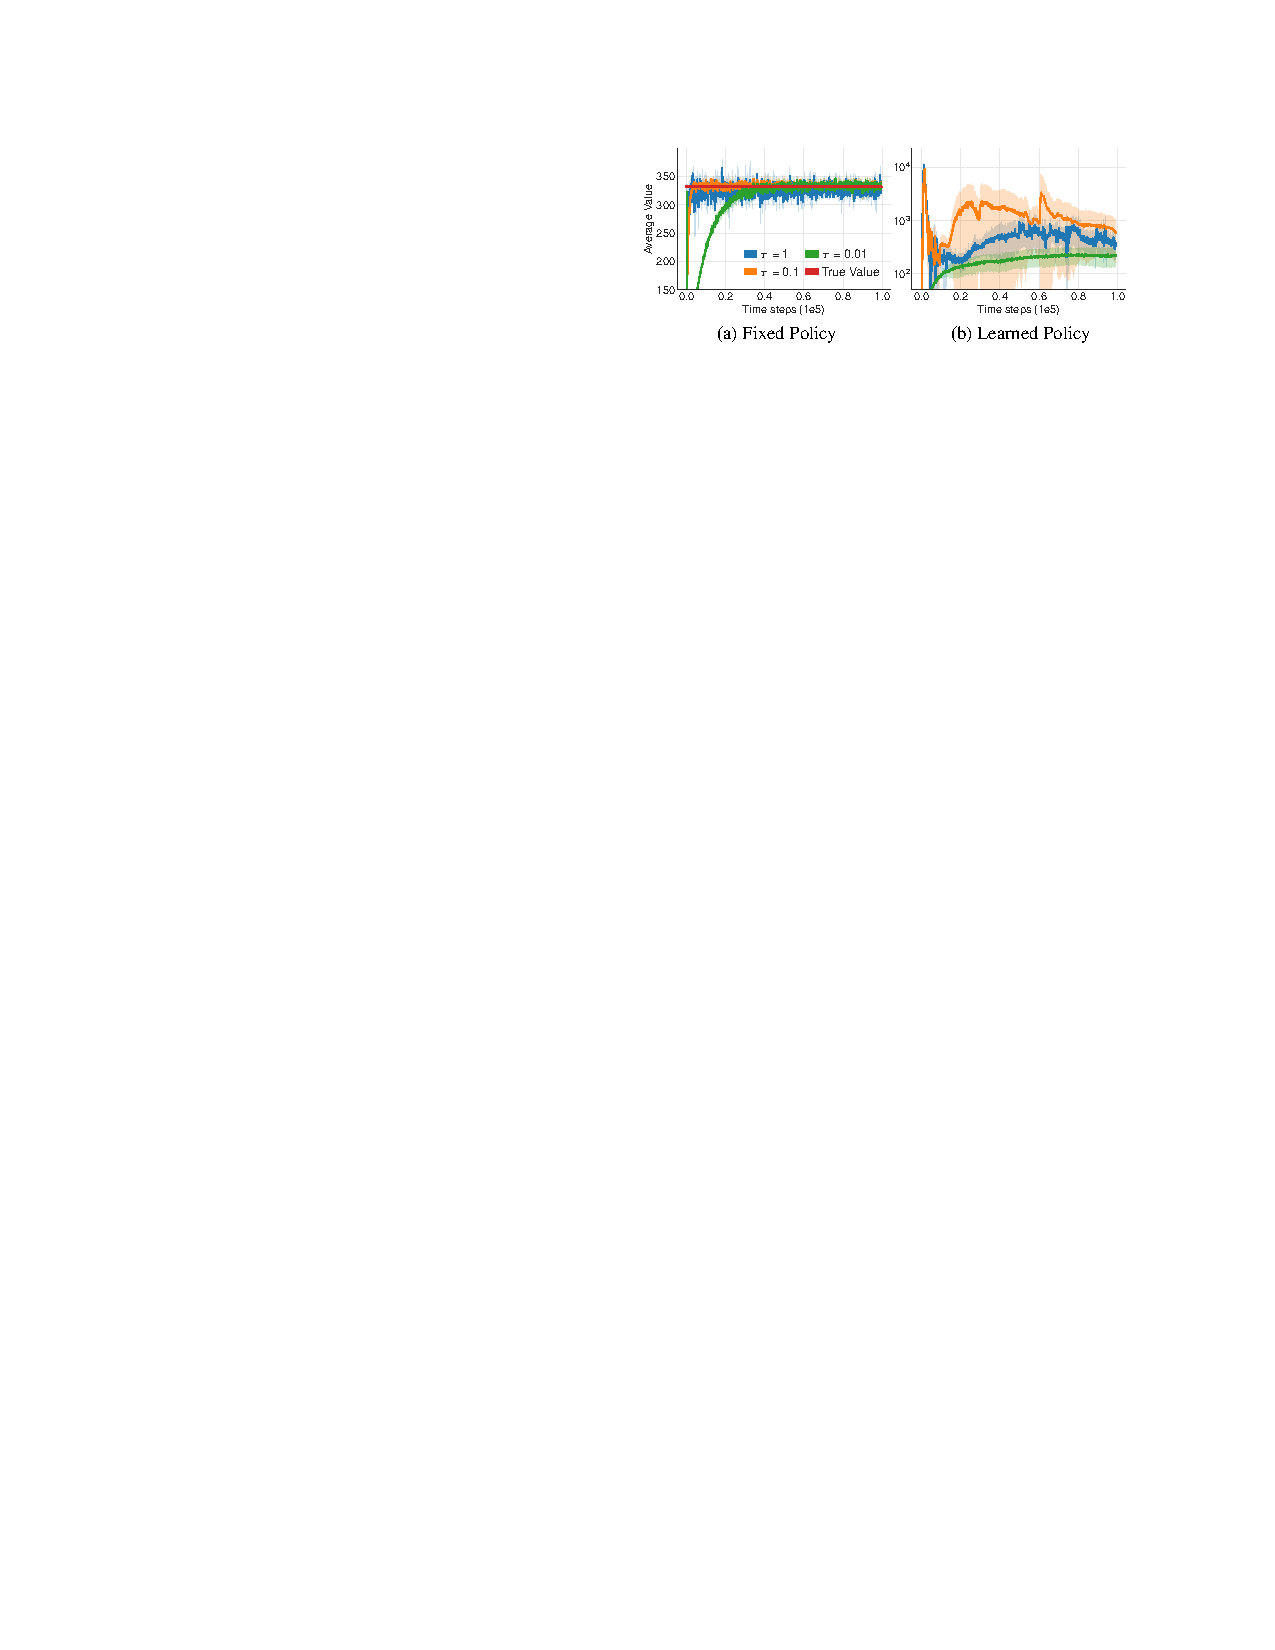
\includegraphics[height=4cm]{fig/lec13/Policy_Update_Frequency_TD3.pdf}
	\caption{Average estimated action value of a randomly selected state on Hopper-v1 environment from \href{https://gym.openai.com/envs/\#mujoco}{OpenAI Gym} (source: S. Fujimoto et al., \textit{Addressing Function Approximation Error in Actor-Critic Methods}, 2018.}
	\label{fig:Policy_Update_Frequency_TD3}
\end{figure}
}	

%%%%%%%%%%%%%%%%%%%%%%%%%%%%%%%%%%%%%%%%%%%%%%%%%%%%%%%%%%%%%
%% Algorithmic Implementation: TD3 %%
%%%%%%%%%%%%%%%%%%%%%%%%%%%%%%%%%%%%%%%%%%%%%%%%%%%%%%%%%%%%%
\frame{%\frametitle{Algo. Implementation: TD3}
\setlength{\algomargin}{0.5em}
\begin{algorithm}[H]
\footnotesize
\SetKwInput{Input}{input} 
\SetKwInput{Output}{output}
\SetKwInput{Init}{init}
\SetKwInput{Param}{parameter}
\Input{diff. det. policy fct. $\bm{\mu}(\bm{x},\bm{\theta})$ and action-value fct. $\hat{q}(\bm{x},\bm{u},\bm{w})$}
\Param{step sizes and filter constant $\{\alpha_{w}, \alpha_{\theta}, \tau\}\in\left\{\mathbb{R}|0<\alpha, \tau<1\right\}$, policy update rate $k_w\in\left\{\mathbb{N}|1\leq k_w\right\}$, target noise $\bm{\Sigma}\in\mathbb{R}^{m \times m}$ and $\bm{c}\in\mathbb{R}^{m}$}
\Init{weights $\bm{w}=\bm{w}_{1}^{-}=\bm{w}_{2}^{-}\in\mathbb{R}^{\zeta}$ and $\bm{\theta}=\bm{\theta}^{-}\in\mathbb{R}^d$ arbitrarily, memory $\bm{\mathcal{D}}$}\pause
 \For{$j=1,2,\ldots,$ episodes}{
		initialize $\bm{x}_0$\; 
		\For{$k=0,1,\ldots, T-1$ time steps}{
			$\bm{u}_k \leftarrow$ apply from $\bm{\mu}(\bm{x}_k, \bm{\theta})$ w/wo noise or from behavior policy\;
			observe $\bm{x}_{k+1}$ and $r_{k+1}$\;
			store tuple $\left\langle \bm{x}_k, \bm{u}_k, r_{k+1}, \bm{x}_{k+1}\right\rangle$ in $\bm{\mathcal{D}}$\;\pause
			sample mini-batch $\bm{\mathcal{D}}_b$ from $\bm{\mathcal{D}}$ (after initial memory warmup)\;
			\For(calculate $Q$-targets){$i=1,\ldots,b$ samples}{
				\lIf{$\bm{x}_{i+1}$ is terminal}{$y_i=r_{i+1}$}
				\Else{
							$\bm{u}'=\mathrm{clip}\left(\bm{\mu}_{\bm{\theta}^{-}}(\bm{x}_{i+1})+\mathrm{clip}\left(\mathcal{N}(\bm{0},\bm{\Sigma}), -\bm{c},\bm{c}\right), \underline{\bm{u}}, \overline{\bm{u}} \right)$\;	
							$y_i= r_{i+1}+ \gamma \min_{l=1,2}\hat{q}(\bm{x}_{i+1},\bm{u}',\bm{w}_{l}^{-})$\;
							}
			}\pause
			fit $\bm{w}_{l}$ on loss $\mathcal{L}(\bm{w}_{l})=[y - \hat{q}(\bm{x}, \bm{u}, \bm{w}_{l})]^2_{\bm{\mathcal{D}}_b}$ with step size $\alpha_{w}$ $\forall \, l$\;\pause
			\If{$k \mod k_w=0$}{
					$\bm{\theta} \leftarrow \bm{\theta} + \alpha_{\theta} [\nabla_{\bm{\theta}}\bm{\mu}(\bm{x},\bm{\theta})\nabla_{\bm{u}}\hat{q}(\bm{x}, \bm{u}, \bm{w}_1)\vert_{\bm{u}=\bm{\mu}_{\bm{\theta}}(\bm{x})}]_{\bm{\mathcal{D}}_b}$\; \pause
					$\bm{w}_{l}^{-} \leftarrow (1-\tau)\bm{w}_{l}^{-}+\tau\bm{w}_{l}, \,\, \bm{\theta}^{-} \leftarrow (1-\tau)\bm{\theta}^{-}+\tau\bm{\theta}$\;
			}
	}
}
\caption{Twin delayed deep deterministic policy gradient (output: parameter vectors $\bm{\theta}^*$ for $\bm{\mu}^*(\bm{x},\bm{\theta}^*)$) and $\bm{w}^*$ for $\hat{q}^*(\bm{x}, \bm{u}, \bm{w}^*))$}
\label{algo:TD3}
\end{algorithm}
}

%%%%%%%%%%%%%%%%%%%%%%%%%%%%%%%%%%%%%%%%%%%%%%%%%%%%%%%%%%%%%%%%%%
\section{Trust Region Policy Optimization (TRPO)} 
%%%%%%%%%%%%%%%%%%%%%%%%%%%%%%%%%%%%%%%%%%%%%%%%%%%%%%%%%%%%%%%%%%
\begin{frame}
\frametitle{Table of Contents}
\tableofcontents[currentsection]
\end{frame}

%%%%%%%%%%%%%%%%%%%%%%%%%%%%%%%%%%%%%%%%%%%%%%%%%%%%%%%%%%%%%
%% Reinterpreting the Policy Gradient for Stochastic Policies (1)%%
%%%%%%%%%%%%%%%%%%%%%%%%%%%%%%%%%%%%%%%%%%%%%%%%%%%%%%%%%%%%%
\setcounter{footnote}{0}
\frame{\frametitle{Reinterpreting the Stochastic Policy Gradient (1)}
\vspace{-0.2cm}
\begin{itemize}
	\item In contrast to the previous two algorithms, we will \hl{focus on stochastic policies} $\pi(\bm{u}|\bm{x})$ in the following.\pause
	\item First, we rewrite the performance metric \eqref{eq:performance_metric_episodic} to obtain
		\begin{equation}
		J_{\pi} =\El{\sum_{k=0}^\infty \gamma^k R_k}{\pi}.
	\end{equation}\vspace{-0.5cm}\pause
	\item Using the advantage $a_\pi(\bm{x},\bm{u})= q_{\pi}(\bm{x},\bm{u})-v_{\pi}(\bm{x})$ we can calculate the performance of an updated policy $\bm{\pi}\rightarrow\tilde{\bm{\pi}}$\footnote{proof from: S. Kakade and J. Langford, \textit{Approximately optimal approximate reinforcement learning}, ICML, vol. 2, pp 267-274, 2002}:
		\begin{equation}
		\label{eq:TRPO_perf_change}
		J_{\tilde{\pi}} =J_{\pi} + \int_\mathcal{X}p^{\tilde{\pi}}(\bm{x})\int_{\mathcal{U}} \tilde{\pi}(\bm{u}|\bm{x})a_\pi(\bm{x},\bm{u}).
	\end{equation}\vspace{-0.5cm}\pause
	\item While for finite MDPs, the policy improvement theorem guaranteed  $J_{\tilde{\pi}} \geq J_{\pi}$ for each policy update, there might be some states where $\int_{\mathcal{U}} \tilde{\pi}(\bm{u}|\bm{x})a_\pi<0$ for continuous MDPs using function approximation. 
\end{itemize}
}

%%%%%%%%%%%%%%%%%%%%%%%%%%%%%%%%%%%%%%%%%%%%%%%%%%%%%%%%%%%%%
%% Reinterpreting the Policy Gradient for Stochastic Policies (2)%%
%%%%%%%%%%%%%%%%%%%%%%%%%%%%%%%%%%%%%%%%%%%%%%%%%%%%%%%%%%%%%
\frame{\frametitle{Reinterpreting the Stochastic Policy Gradient  (2)}
\begin{itemize}
	\item For easier calculation, we introduce a local approximation to \eqref{eq:TRPO_perf_change}
	\begin{equation}
		\mathcal{L}_{\pi}(\tilde{\pi}) =J_{\pi} + \int_\mathcal{X}p^{\pi}(\bm{x})\int_{\mathcal{U}} \tilde{\pi}(\bm{u}|\bm{x})a_\pi(\bm{x},\bm{u})
	\end{equation}
	where $p^{\pi}(\bm{x})$ is used instead of $p^{\tilde{\pi}}(\bm{x})$, i.e., neglecting the state distribution change due to a policy update.\pause
	\item For any parametrized and differentiable policy $\pi_{\bm{\theta}}(\bm{u}|\bm{x})$, it can be shown that
	\begin{equation}
	\begin{split}
		 \mathcal{L}(\pi_{\bm{\theta}_0}) &= J(\pi_{\bm{\theta}_0}),\\
		\nabla_{\bm{\theta}}\mathcal{L}_{\pi_{\bm{\theta}_0}}(\pi_{\bm{\theta}})|_{\bm{\theta}=\bm{\theta}_0} &= \nabla_{\bm{\theta}}J(\pi_{\bm{\theta}})|_{\bm{\theta}=\bm{\theta}_0}
	\end{split}	
	\end{equation}
	for any initial parameter set $\bm{\theta}_0$.\pause
	 \item For a sufficiently small step size, improving $\mathcal{L}_{\pi_{\bm{\theta}_0}}$ will also improve $J$. \pause
\end{itemize}
\begin{block}{}
However, we do not know how much the actual stochastic policy will change while moving through the parameter space. Hence, we do not have a good decision basis to choose the policy gradient step size.   
\end{block}
}

%%%%%%%%%%%%%%%%%%%%%%%%%%%%%%%%%%%%%%%%%%%%%%%%%%%%%%%%%%%%%
%% Adding a Trust Region Constraint (1)%%
%%%%%%%%%%%%%%%%%%%%%%%%%%%%%%%%%%%%%%%%%%%%%%%%%%%%%%%%%%%%%
\frame{\frametitle{Adding a Trust Region Constraint (1)}
\begin{itemize}
	\item From the previous discussion it can be concluded that we want a \hl{metric describing how much a policy is changed in the action space when updating the policy in the parameter space}. \pause 
	\item Against this background, we make use of the \hl{Kullback-Leibler divergence} (also called relative entropy)
	\begin{equation}
		D_{\mathrm{KL}}(P \parallel Q) = \int_{-\infty}^\infty p(x) \log\left(\frac{p(x)}{q(x)}\right)\, \mathrm{d}x
	\end{equation}
	defined for continuous distributions $P$ and $Q$ with their probability densities $p$ and $q$. \pause
	\item Example: for two multivariate Gaussian distributions of equal dimensions $d$, with means $\bm{\mu}_0, \bm{\mu}_1$ and with (non-singular) covariance matrix $\bm{\Sigma}_0, \bm{\Sigma}_1$ we receive
\end{itemize}
	\small
	\begin{align*}
D_{\mathrm{KL}}\left(\mathcal{N}_0 \parallel \mathcal{N}_1\right) =  \frac{1}{2}&\left(\mathrm{tr}\left(\bm{\Sigma}_1^{-1}\bm{\Sigma}_0\right) + \left(\bm{\mu}_1 - \bm{\mu}_0\right)\T \bm{\Sigma}_1^{-1}\left(\bm{\mu}_1 - \bm{\mu}_0\right) \right. \\ &\left.- d + \ln\left(\frac{\det\bm{\Sigma}_1}{\det\bm{\Sigma}_0}\right) \right).		
	\end{align*}
	\normalsize
}

%%%%%%%%%%%%%%%%%%%%%%%%%%%%%%%%%%%%%%%%%%%%%%%%%%%%%%%%%%%%%
%% Adding a Trust Region Constraint (2)%%
%%%%%%%%%%%%%%%%%%%%%%%%%%%%%%%%%%%%%%%%%%%%%%%%%%%%%%%%%%%%%
\frame{\frametitle{Adding a Trust Region Constraint (2)}
\begin{itemize}
	\item The \hl{trust region policy optimization (TRPO)} updates the policy parameters while constraining the KL divergence between the new and the old policy distribution:
	\begin{equation}
	\label{eq:TRPO_opt_prob}
	\begin{split}
		 &\max_{\bm{\theta}}  \, \mathcal{L}_{\bm{\theta}_k}(\bm{\theta}),\\
		 \mbox{s.t.} \quad\quad  & \overline{D}_{\mathrm{KL}}(\bm{\theta}_k, \bm{\theta})\leq\kappa
	\end{split}
	\end{equation}\pause
	with 
\end{itemize}
\vspace{0.15cm}
	\begin{equation*}
\overline{D}_{\mathrm{KL}}(\bm{\theta}_k, \bm{\theta})=\overline{D}_{\mathrm{KL}}(\pi_{\bm{\theta}_k}, \pi_{\bm{\theta}})=\El{D_{\mathrm{KL}}(\pi_{\bm{\theta}_k}(\cdot|\bm{X}) \parallel \pi_{\bm{\theta}}(\cdot|\bm{X}))}{\pi_{\bm{\theta}_k}}.
	\end{equation*}
	\vspace{-0.25cm}\pause
\begin{itemize}
	\item Hence, we want to \hl{limit the average KL divergence w.r.t. the states visited by the old policy}.\pause
	\item The constraint $\kappa$ is a TRPO hyperparameter (typically $\kappa<<1$). \pause
	\item Although \eqref{eq:TRPO_opt_prob}  does not provide any formal convergence guarantee, we at least have a link between changes in the parameter and policy distribution space. Therefore, \hl{we can use this tool to prevent erratic policy changes}.  
\end{itemize}
}

%%%%%%%%%%%%%%%%%%%%%%%%%%%%%%%%%%%%%%%%%%%%%%%%%%%%%%%%%%%%%
%% Sample-Based Estimation of the Objective and Constraint%%
%%%%%%%%%%%%%%%%%%%%%%%%%%%%%%%%%%%%%%%%%%%%%%%%%%%%%%%%%%%%%
\frame{\frametitle{Sample-Based Objective and Constraint Estimation (1)}
\begin{itemize}
	\item To actually solve \eqref{eq:TRPO_opt_prob} we will make use of samplings from \hl{Monte-Carlo rollouts}.\pause
	\item Expanding the objective yields
	\begin{equation}
		\max_{\bm{\theta}}  \, \mathcal{L}_{\bm{\theta}_k}(\bm{\theta})= \max_{\bm{\theta}} \, J_{\pi_k} + \int_\mathcal{X}p^{\pi_k}(\bm{x})\int_{\mathcal{U}} \pi_{\bm{\theta}}(\bm{u}|\bm{x})a_{\pi_k}(\bm{x},\bm{u}).
	\end{equation}\pause
	\item The first term $J_{\pi_k}$ can be dropped, since it is irrelevant for the optimization result (constant).\pause
	\item Using samples we can approximate $\int_\mathcal{X}p^{\pi_k}(\bm{x})\approx\frac{1}{1-\gamma}\El{\bm{X}}{\pi_{\bm{\theta}_k}}$.\pause
	\item Moreover, $\int_{\mathcal{U}} \pi_{\bm{\theta}}(\bm{u}|\bm{x})a_{\pi_k}(\bm{x},\bm{u})\approx\El{\frac{\pi_{\bm{\theta}}(\bm{U}|\bm{X})}{\pi_{\bm{\theta}_k}(\bm{U}|\bm{X})}a_{\pi_k}(\bm{X},\bm{U})}{\pi_{\bm{\theta}_k}}$ is also approximated applying importance sampling based on data from the old policy.\pause
	\item Hence, the sampled objective is
	\begin{equation}
		\max_{\bm{\theta}} \,\El{\frac{\pi_{\bm{\theta}}(\bm{U}|\bm{X})}{\pi_{\bm{\theta}_k}(\bm{U}|\bm{X})}a_{\pi_k}(\bm{X},\bm{U})}{\pi_{\bm{\theta}_k}}.
	\end{equation}
\end{itemize}
}

%%%%%%%%%%%%%%%%%%%%%%%%%%%%%%%%%%%%%%%%%%%%%%%%%%%%%%%%%%%%%
%% Smooth Policy Updates via TRPO %%
%%%%%%%%%%%%%%%%%%%%%%%%%%%%%%%%%%%%%%%%%%%%%%%%%%%%%%%%%%%%%
\frame{\frametitle{Smooth Policy Updates via TRPO}
\begin{figure}
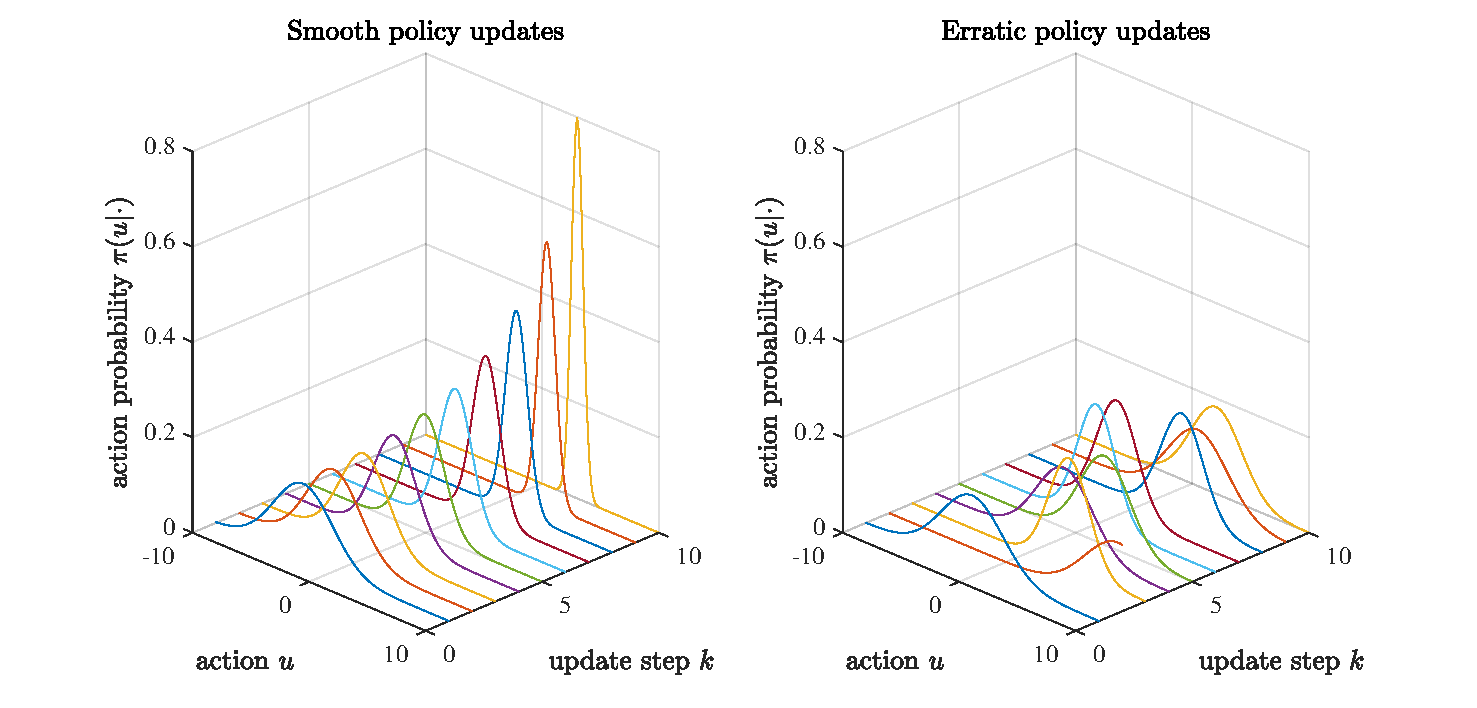
\includegraphics[height=5.75cm]{fig/lec13/TRPO_Style_Updates.pdf}
\caption{Simplified representation of the policy evolution for a scalar action given some fixed state. Left: TRPO-style updates finding the optimal action with increasing probability. Right: Unmonitored policy distributions not converging towards an optimal policy ('policy chattering').}
\label{fig:TRPO_Style_Updates}
\end{figure}
}	

%%%%%%%%%%%%%%%%%%%%%%%%%%%%%%%%%%%%%%%%%%%%%%%%%%%%%%%%%%%%%
%% Sample-Based Estimation of the Objective and Constraint%%
%%%%%%%%%%%%%%%%%%%%%%%%%%%%%%%%%%%%%%%%%%%%%%%%%%%%%%%%%%%%%
\frame{\frametitle{Sample-Based Objective and Constraint Estimation (2)}
\begin{itemize}
	\item Applying the previous sample-based estimation we obtain
\end{itemize}
\vspace{0.15cm}
		\begin{equation}
	\label{eq:TRPO_opt_prob_sample}
	\begin{split}
		 &\bm{\theta}_{k+1} = \argmax_{\bm{\theta}} \,\El{\frac{\pi_{\bm{\theta}}(\bm{U}|\bm{X})}{\pi_{\bm{\theta}_k}(\bm{U}|\bm{X})}a_{\pi_k}(\bm{X},\bm{U})}{\pi_{\bm{\theta}_k}},\\
		 \mbox{s.t.} \quad\quad  & \El{D_{\mathrm{KL}}(\pi_{\bm{\theta}_k}(\cdot|\bm{X}) \parallel \pi_{\bm{\theta}}(\cdot|\bm{X}))}{{\pi_{\bm{\theta}_k}}}\leq\kappa.
	\end{split}
	\end{equation}
	\vspace{-0.25cm}
\begin{itemize}\pause
	\item Hence, we have a \hl{three-step procedure} for each TRPO update:\pause
\end{itemize}
\begin{enumerate}
	\item Use Monte-Carlo simulations based on the old policy to obtain data.\pause
	\item Use the data to construct \eqref{eq:TRPO_opt_prob_sample}.\pause
	\item Solve the constrained optimization problem to update the policy parameter vector. 
\end{enumerate}\pause
\begin{block}{}
Solving  \eqref{eq:TRPO_opt_prob_sample} is generally a nonlinear optimization problem. The original TRPO implementation uses a local objective and constraint approximation together with conjugate gradient and line search algorithms. However, many other constrained-nonlinear solvers are also applicable.
\end{block}
}

%%%%%%%%%%%%%%%%%%%%%%%%%%%%%%%%%%%%%%%%%%%%%%%%%%%%%%%%%%%%%
%% Generalized Advantage Estimation %%
%%%%%%%%%%%%%%%%%%%%%%%%%%%%%%%%%%%%%%%%%%%%%%%%%%%%%%%%%%%%%
\frame{\frametitle{Generalized Advantage Estimation}
\setcounter{footnote}{0}
\begin{itemize}
	\item Having data $\left\langle \bm{x}, \bm{u}, r, \bm{x}'\right\rangle$ in $\bm{\mathcal{D}}$ from a Monte Carlo rollout available, an imporant problem is to estimate $a_{\pi_k}(\bm{x},\bm{u})$ in \eqref{eq:TRPO_opt_prob_sample}.\pause
	\item A particular suggestion in the TRPO context is to use a \hl{generalized advantage estimator (GAE)} \footnote{cf. J. Schulmann et al., \textit{High Dimensional Continuous Control Using Generalized Advantage Estimation}, \href{https://arxiv.org/abs/1506.02438}{https://arxiv.org/abs/1506.02438}, 2015} defined as
	\begin{equation}
	\label{eq:GAE}
		\hat{a}_k^{(\gamma, \lambda)} = \sum_{i=0}^\infty (\gamma\lambda)^i\delta_{k+i}.
	\end{equation}\pause
	\item Here, $\delta_{k}=r_k+\gamma v(\bm{x}_{k+1})-v(\bm{x}_{k})$ is a single advantage sample.\pause
	\item Hence, the GAE is the exponentially-weighted average of the discounted advantage samples with an additional weighting $\lambda$.\pause
	\item Similar formulation compared to TD$(\lambda)$ but instead of the state value the estimator's target is the advantage. \pause
	\item The choice of $(\gamma\lambda)$ trade-offs the bias and variance of the estimator. 
\end{itemize}	
}

%%%%%%%%%%%%%%%%%%%%%%%%%%%%%%%%%%%%%%%%%%%%%%%%%%%%%%%%%%%%%
%% Summary %%
%%%%%%%%%%%%%%%%%%%%%%%%%%%%%%%%%%%%%%%%%%%%%%%%%%%%%%%%%%%%%
\frame{\frametitle{TRPO Summary}
\vspace{-0.1cm}
The TRPO's key facts are:
\begin{itemize}
	\item The TRPO constrains policy distribution changes when updating the policy parameters (for stochastic policies and on-policy learning).\pause
	\item The objective is to enable a monotonically improving learning process.\pause
	\item Using trust regions, erratic policy updates should be prevented.\pause
\end{itemize}	
The TRPO's main hurdles are:
\begin{itemize}
	\item Constructing the objective function and constraint requires Monte Carlo rollouts (time consuming, data inefficient).\pause
	\item When the sampled optimization problem is set up, a nonlinear and constrained optimization step is required (no simple policy gradient).\pause
	\item For speedy implementations, only approximate solutions of the TRPO problem are possible.
\end{itemize}\pause	
\begin{block}{}
We will not provide any specific TRPO implementation suggestion at this point, since this is rather cumbersome. Instead we will move forward to a similar algorithm which is pursuing the same goal (prevent erratic policy changes) with a much simpler implementation.  
\end{block}
}

%%%%%%%%%%%%%%%%%%%%%%%%%%%%%%%%%%%%%%%%%%%%%%%%%%%%%%%%%%%%%%%%%%
\section{Proximal Policy Optimization (PPO)} 
%%%%%%%%%%%%%%%%%%%%%%%%%%%%%%%%%%%%%%%%%%%%%%%%%%%%%%%%%%%%%%%%%%
\begin{frame}
\frametitle{Table of Contents}
\tableofcontents[currentsection]
\end{frame}

%%%%%%%%%%%%%%%%%%%%%%%%%%%%%%%%%%%%%%%%%%%%%%%%%%%%%%%%%%%%%
%% Background and Motivation %%
%%%%%%%%%%%%%%%%%%%%%%%%%%%%%%%%%%%%%%%%%%%%%%%%%%%%%%%%%%%%%
\frame{\frametitle{Background and Motivation}
\begin{itemize}
	\item The upcoming \hl{proximal policy optimization (PPO)} algorithm tries to mimic the constrained TRPO problem based on related unconstrained problems. 
\end{itemize}	
\vspace{0.15cm}
		\begin{equation*}
	\begin{split}
		 &\bm{\theta}_{k+1} = \argmax_{\bm{\theta}} \,\El{\frac{\pi_{\bm{\theta}}(\bm{U}|\bm{X})}{\pi_{\bm{\theta}_k}(\bm{U}|\bm{X})}a_{\pi_k}(\bm{X},\bm{U})}{\pi_{\bm{\theta}_k}},\\
		 \mbox{s.t.} \quad\quad  & \El{D_{\mathrm{KL}}(\pi_{\bm{\theta}_k}(\cdot|\bm{X}) \parallel \pi_{\bm{\theta}}(\cdot|\bm{X}))}{{\pi_{\bm{\theta}_k}}}\leq\kappa.
	\end{split}
	\end{equation*}
\vspace{-0.25cm}\pause
\begin{itemize}
	\item Hence, the objective will be reformulated to incorporate mechanisms preventing excessively large variations of the policy distribution during a parameter update (leading to an updated policy with sufficient proximity to the old one).  \pause
	\item Moreover, PPO incorporates two variants which we will discuss:
	\begin{enumerate}
	\item Clipping the surrogate objective,\pause
	\item Adaptive tuning of a KL-associated penalty coefficient.
\end{enumerate}
\end{itemize}
}

%%%%%%%%%%%%%%%%%%%%%%%%%%%%%%%%%%%%%%%%%%%%%%%%%%%%%%%%%%%%%
%% Clipped Surrogate Objective %%
%%%%%%%%%%%%%%%%%%%%%%%%%%%%%%%%%%%%%%%%%%%%%%%%%%%%%%%%%%%%%
\frame{\frametitle{Clipped Surrogate Objective}
\begin{itemize}
	\item The first approach is based on the following objective:
\end{itemize}
\vspace{0.25cm}
\small
\begin{equation}
\label{eq:PPO_CSO}
		\hspace{-0.2cm}\El{\min\left\{\frac{\pi_{\bm{\theta}}(\bm{U}|\bm{X})}{\pi_{\bm{\theta}_k}(\bm{U}|\bm{X})}a_{\pi_k}(\bm{X},\bm{U}), \mathrm{clip}\left(\frac{\pi_{\bm{\theta}}(\bm{U}|\bm{X})}{\pi_{\bm{\theta}_k}(\bm{U}|\bm{X})}, 1-\epsilon, 1+\epsilon\right)a_{\pi_k}(\bm{X},\bm{U})\right\}}{\pi_{\bm{\theta}_k}}.
\end{equation}\pause
\normalsize
\begin{itemize}
	\item Above, $\epsilon<1$ is a PPO hyperparameter serving as a regularizer.\pause
	\item The first element of $\min\{\cdot\}$ is the previous TPRO objective.\pause
	\item The second element of $\min\{\cdot\}$ modifies the surrogate objective by clipping the importance sampling ratio $\pi_{\bm{\theta}}/\pi_{\bm{\theta}_k}$.\pause
	\item The latter should remove the incentive for moving the importance sampling ratio outside of the interval $[1-\epsilon, 1+\epsilon]$.\pause
	\item The modified objective is therefore a lower bound of the unclipped TRPO objective. 
\end{itemize}
}

%%%%%%%%%%%%%%%%%%%%%%%%%%%%%%%%%%%%%%%%%%%%%%%%%%%%%%%%%%%%%
%% Clipped Surrogate Objective: Positive Advantage %%
%%%%%%%%%%%%%%%%%%%%%%%%%%%%%%%%%%%%%%%%%%%%%%%%%%%%%%%%%%%%%
\frame{\frametitle{Clipped Surrogate Objective: Positive Advantage}
\begin{itemize}
	\item Consider a single sample $(\bm{x}, \bm{u})$ with a \hl{positive advantage} $a_{\pi_k}(\bm{x},\bm{u})$:\pause
\end{itemize}
\vspace{0.1cm}
\begin{equation*}
		\max_{\bm{\theta}}\,\min\left\{\frac{\pi_{\bm{\theta}}(\bm{u}|\bm{x})}{\pi_{\bm{\theta}_k}(\bm{u}|\bm{x})}a_{\pi_k}(\bm{x},\bm{u}), \mathrm{clip}\left(\frac{\pi_{\bm{\theta}}(\bm{u}|\bm{x})}{\pi_{\bm{\theta}_k}(\bm{u}|\bm{x})}, 1-\epsilon, 1+\epsilon\right)a_{\pi_k}(\bm{x}, \bm{u})\right\}.
\end{equation*}\pause
\begin{itemize}
	\item Because the advantage is positive, the objective will increase if the action becomes more likely, i.e., if $\pi_{\bm{\theta}}(\bm{u}|\bm{x})$ increases.\pause
	\item If $\pi_{\bm{\theta}}(\bm{u}|\bm{x}) > (1+\epsilon)\pi_{\bm{\theta}_k}(\bm{u}|\bm{x})$ the clipping becomes active.\pause
	\item Hence, the objective reduces to
	\begin{equation*}
		\max_{\bm{\theta}}\,\min\left\{\frac{\pi_{\bm{\theta}}(\bm{u}|\bm{x})}{\pi_{\bm{\theta}_k}(\bm{u}|\bm{x})},  1+\epsilon\right\}a_{\pi_k}(\bm{x},\bm{u}).
\end{equation*}\pause
	\item Due to the $\min\{\cdot\}$ operator, the entire objective is therefore limited to $(1+\epsilon)a_{\pi_k}(\bm{x},\bm{u})$.\pause
	\item Interpretation: the new policy does not benefit from going further away from the old policy.
\end{itemize}
}

%%%%%%%%%%%%%%%%%%%%%%%%%%%%%%%%%%%%%%%%%%%%%%%%%%%%%%%%%%%%%
%% Clipped Surrogate Objective: Negative Advantage %%
%%%%%%%%%%%%%%%%%%%%%%%%%%%%%%%%%%%%%%%%%%%%%%%%%%%%%%%%%%%%%
\frame{\frametitle{Clipped Surrogate Objective: Negative Advantage}
\begin{itemize}
	\item Consider a single sample $(\bm{x}, \bm{u})$ with a \hl{negative advantage} $a_{\pi_k}(\bm{x},\bm{u})$:\pause
\end{itemize}
\vspace{0.1cm}
\begin{equation*}
		\max_{\bm{\theta}}\,\min\left\{\frac{\pi_{\bm{\theta}}(\bm{u}|\bm{x})}{\pi_{\bm{\theta}_k}(\bm{u}|\bm{x})}a_{\pi_k}(\bm{x},\bm{u}), \mathrm{clip}\left(\frac{\pi_{\bm{\theta}}(\bm{u}|\bm{x})}{\pi_{\bm{\theta}_k}(\bm{u}|\bm{x})}, 1-\epsilon, 1+\epsilon\right)a_{\pi_k}(\bm{x},\bm{u})\right\}.
\end{equation*}\pause
\begin{itemize}
	\item Because the advantage is negative, the objective will increase if the action becomes less likely, i.e., if $\pi_{\bm{\theta}}(\bm{u}|\bm{x})$ decreases.\pause
	\item If $\pi_{\bm{\theta}}(\bm{u}|\bm{x}) < (1-\epsilon)\pi_{\bm{\theta}_k}(\bm{u}|\bm{x})$ the clipping becomes active.\pause
	\item Hence, the objective reduces to
	\begin{equation*}
		\max_{\bm{\theta}}\,\max\left\{\frac{\pi_{\bm{\theta}}(\bm{u}|\bm{x})}{\pi_{\bm{\theta}_k}(\bm{u}|\bm{x})},  1-\epsilon\right\}a_{\pi_k}(\bm{x},\bm{u}).
\end{equation*}\pause
	\item Due to the $\max\{\cdot\}$ operator, the entire objective is limited to $(1-\epsilon)a_{\pi_k}(\bm{x},\bm{u})$.\pause
	\item Interpretation: the new policy does not benefit from going further away from the old policy.
\end{itemize}
}

%%%%%%%%%%%%%%%%%%%%%%%%%%%%%%%%%%%%%%%%%%%%%%%%%%%%%%%%%%%%%
%% Adaptive KL Penalty %%
%%%%%%%%%%%%%%%%%%%%%%%%%%%%%%%%%%%%%%%%%%%%%%%%%%%%%%%%%%%%%
\frame{\frametitle{Adaptive KL Penalty}
\begin{itemize}
	\item The second PPO variant makes use of the following KL-penalized objective
\end{itemize}
\vspace{0.15cm}
\small
	\begin{equation}
	\label{eq:PPO_AKP}
      \El{\frac{\pi_{\bm{\theta}}(\bm{U}|\bm{X})}{\pi_{\bm{\theta}_k}(\bm{U}|\bm{X})}a_{\pi_k}(\bm{X},\bm{U})-\beta D_{\mathrm{KL}}(\pi_{\bm{\theta}_k}(\cdot|\bm{X}) \parallel \pi_{\bm{\theta}}(\cdot|\bm{X}))}{\pi_{\bm{\theta}_k}}.		
	\end{equation}
	\normalsize\pause
	\vspace{-0.25cm}
\begin{itemize}
	\item Transfers the KL-based constraint into a penalty for large policy distribution changes.\pause
	\item The parameter $\beta$ weights the penalty against the policy improvement.\pause
	\item The original PPO implementation suggests an adaptive tuning of $\beta$ w.r.t. the sampled average KL divergence $\overline{D}_{\mathrm{KL}}(\bm{\theta}_k, \bm{\theta})$ estimated from previous experience
	\begin{equation}
	\begin{split}
		  \overline{D}_{\mathrm{KL}}(\bm{\theta}_k, \bm{\theta}) < \overline{D}^*_{\mathrm{KL}}: &\quad \beta \leftarrow \beta/2,\\ 
			\overline{D}_{\mathrm{KL}}(\bm{\theta}_k, \bm{\theta}) > \overline{D}^*_{\mathrm{KL}}: &\quad \beta \leftarrow \beta \cdot 2.
	\end{split}	
	\end{equation}
	with some target value of the KL divergence $\overline{D}^*_{\mathrm{KL}}$ (additional hyperparameter). 
\end{itemize}
}

%%%%%%%%%%%%%%%%%%%%%%%%%%%%%%%%%%%%%%%%%%%%%%%%%%%%%%%%%%%%%
%% Algorithmic Implementation: PPO %%
%%%%%%%%%%%%%%%%%%%%%%%%%%%%%%%%%%%%%%%%%%%%%%%%%%%%%%%%%%%%%
\frame{\frametitle{Algo. Implementation: PPO}
\setlength{\algomargin}{0.5em}
\begin{algorithm}[H]
\small
\SetKwInput{Input}{input} 
\SetKwInput{Output}{output}
\SetKwInput{Init}{init}
\SetKwInput{Param}{parameter}
\Input{diff. stochastic policy fct. $\pi(\bm{u}|\bm{x},\bm{\theta})$ and value fct. $\hat{v}(\bm{x},\bm{w})$}
\Param{step sizes $\{\alpha_{w}, \alpha_{\theta}\}\in\left\{\mathbb{R}|0<\alpha\right\}$}
\Init{weights $\bm{w}\in\mathbb{R}^{\zeta}$ and $\bm{\theta}\in\mathbb{R}^d$ arbitrarily, memory $\bm{\mathcal{D}}$}\pause
 \For{$j=1,2,\ldots,$ (sub-)episodes}{
		initialize $\bm{x}_0$ (if new episode)\; 
		collect a set of tuples $\left\langle \bm{x}_k, \bm{u}_k, r_{k+1}, \bm{x}_{k+1}\right\rangle$ by running $\pi(\bm{u}|\bm{x},\bm{\theta}_j)$\;\pause
		store them in $\bm{\mathcal{D}}$\;\pause
		estimate the advantage $\hat{a}_{\pi_j}(\bm{x},\bm{u})$ based on $\hat{v}(\bm{x},\bm{w}_j)$ and $\bm{\mathcal{D}}$ (e.g., GAE)\;\pause
		$\bm{\theta}_{j+1}\leftarrow$ policy gradient update on \eqref{eq:PPO_CSO} or \eqref{eq:PPO_AKP}\;\pause
		$\bm{w}_{j+1}\leftarrow$ minimizing the mean-squared TD errors using $\bm{\mathcal{D}}$\;\pause
		delete entries in $\bm{\mathcal{D}}$\;
	}
\caption{Proximal policy optimization (output: parameter vectors $\bm{\theta}^*$ for $\pi^*(\bm{u}|\bm{x},\bm{\theta}^*)$) and $\bm{w}^*$ for $\hat{v}^*(\bm{x}, \bm{w}^*))$}
\label{algo:PPO}
\end{algorithm}
}

%%%%%%%%%%%%%%%%%%%%%%%%%%%%%%%%%%%%%%%%%%%%%%%%%%%%%%%%%%%%%
%% Some PPO Remarks %%
%%%%%%%%%%%%%%%%%%%%%%%%%%%%%%%%%%%%%%%%%%%%%%%%%%%%%%%%%%%%%
\frame{\frametitle{Some PPO Remarks}
\setcounter{footnote}{0}
\begin{itemize}
	\item Clipping the surrogate objective \eqref{eq:PPO_CSO} was reported to achieve higher performances than the KL penalty \eqref{eq:PPO_AKP}.\footnote{cf. original PPO paper results by J. Schulman et al., \textit{Proximal Policy Optimization Algorithms}, \href{https://arxiv.org/abs/1707.06347}{https://arxiv.org/abs/1707.06347}, 2017}\pause
	\item Like TRPO, PPO is an on-policy algorithm. Hence, the memory $\bm{\mathcal{D}}$ is not a rolling replay buffer (cf. off-policy algorithms like DQN, DDPG or TD3) but a \hl{rollout buffer} using one fixed policy.\pause
	\item These rollouts are likely to result in an increased sample demand either using a simulator or a real experiment.\pause
\end{itemize}
\begin{block}{}
Although PPO is derived from a TRPO background pursuing monotonically increasing policy performance, its realization is based on multiple heuristics and approximations. Hence, there is no guarantee on achieving this goal and the specific performance of the PPO algorithm must be evaluated empirically given a certain application.  
\end{block}
}

%%%%%%%%%%%%%%%%%%%%%%%%%%%%%%%%%%%%%%%%%%%%%%%%%%%%%%%%%%%%%
%% Exemplary Performance Comparison %%
%%%%%%%%%%%%%%%%%%%%%%%%%%%%%%%%%%%%%%%%%%%%%%%%%%%%%%%%%%%%%
\frame{\frametitle{Exemplary Performance Comparison}
\begin{figure}
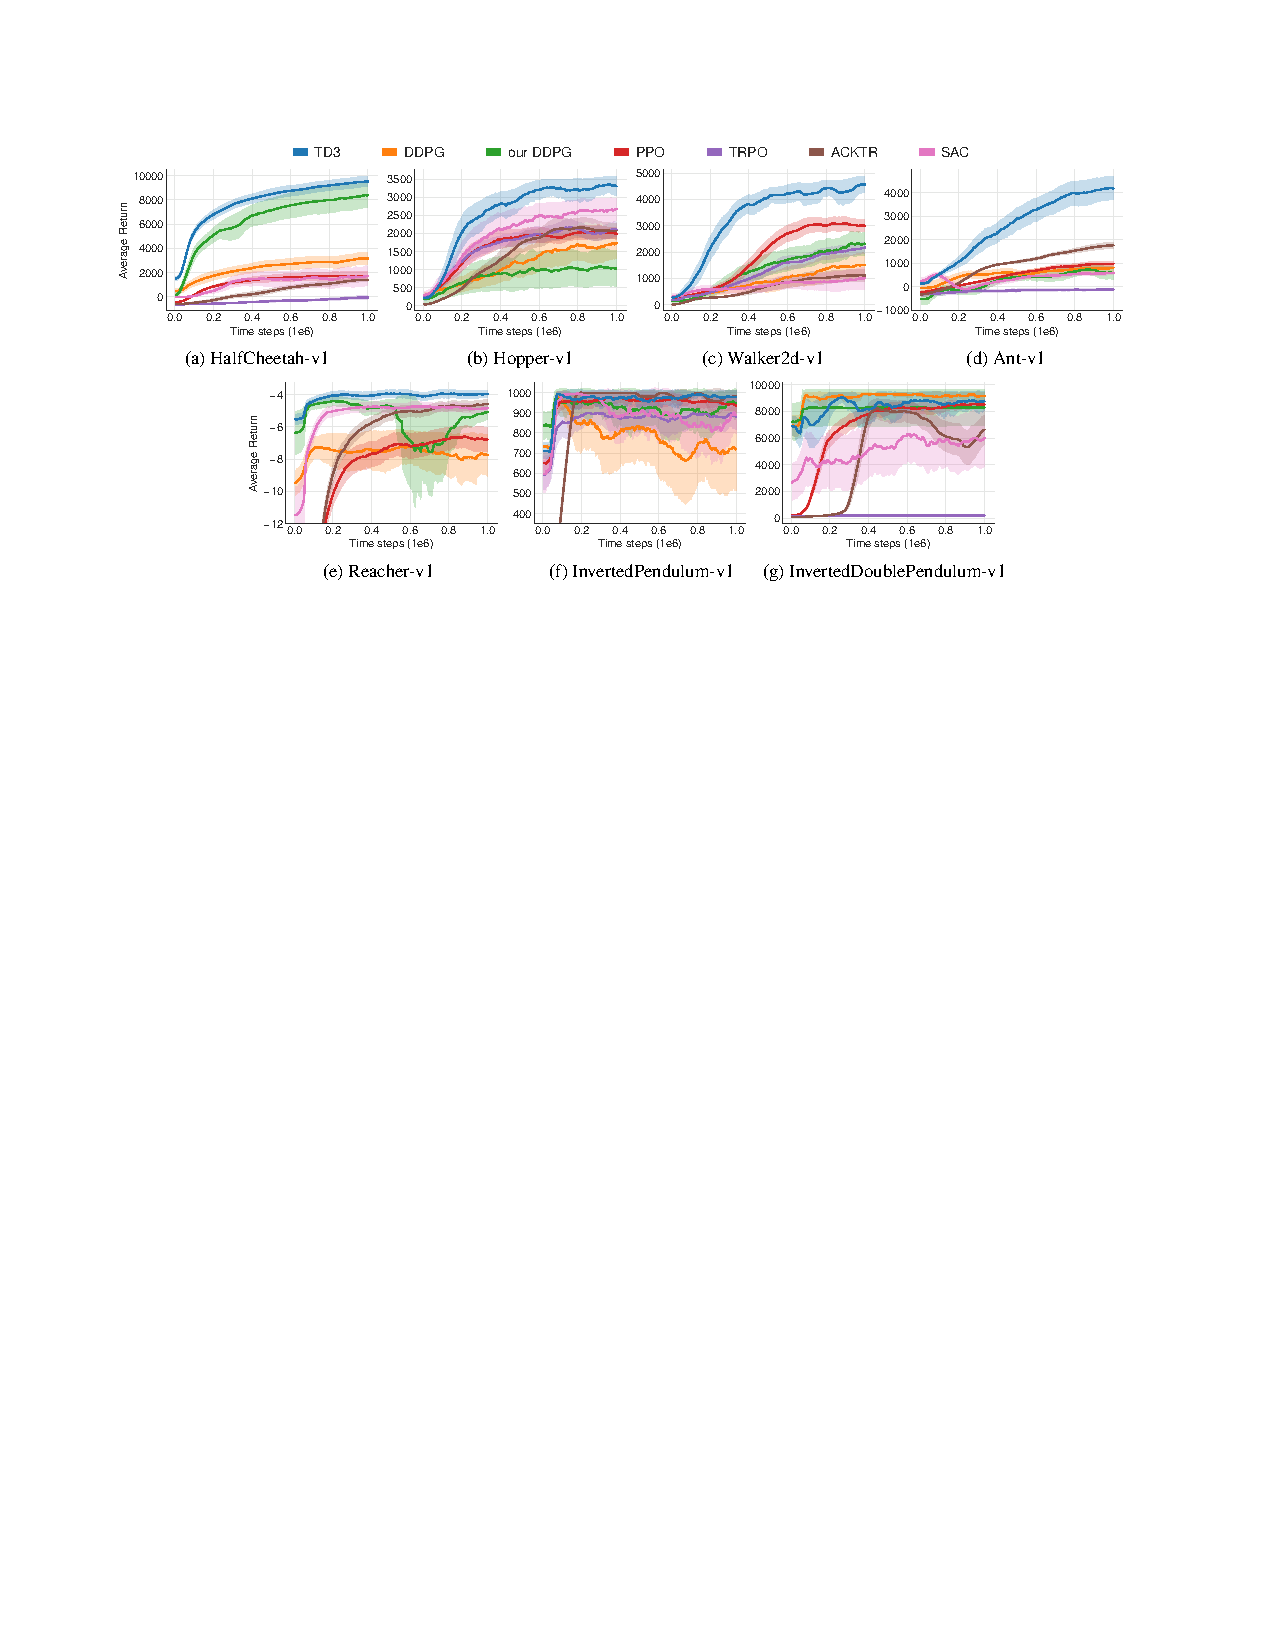
\includegraphics[height=5.25cm]{fig/lec13/Algo_Compare.pdf}
\caption{Learning curves for \href{https://gym.openai.com/envs/\#mujoco}{OpenAI Gym} continuous control tasks. The shaded region represents half a standard deviation of the average evaluation over ten trials (source: S. Fujimoto et al., \textit{Addressing Function Approximation Error in Actor-Critic Methods}, 2018).}
\label{fig:Algo_Compare}
\end{figure}
}	

%%%%%%%%%%%%%%%%%%%%%%%%%%%%%%%%%%%%%%%%%%%%%%%%%%%%%%%%%%%%%
%% Outlook: Other Contempororay Algorithms (1)%%
%%%%%%%%%%%%%%%%%%%%%%%%%%%%%%%%%%%%%%%%%%%%%%%%%%%%%%%%%%%%%
\frame{\frametitle{Outlook: Other Contemporary Algorithms (1)}
The selection of algorithms appears endless:
\begin{itemize}
	\item DQN variants such as
	\begin{itemize}
		\item \href{https://arxiv.org/abs/1511.06581}{(Prioritized) dueling DQN}
		\item \href{https://arxiv.org/abs/1706.10295}{Noisy DQN}
		\item \href{https://arxiv.org/abs/1707.06887}{Distributional DQN}
	\end{itemize}\pause
	\item \href{https://www.aaai.org/ocs/index.php/AAAI/AAAI18/paper/viewFile/17204/16680}{Rainbow} (combining multiple DQN extensions)\pause
	\item \href{https://arxiv.org/abs/1801.01290}{Soft actor-critic (SAC)}\pause
	\item \href{https://proceedings.neurips.cc/paper/2017/file/361440528766bbaaaa1901845cf4152b-Paper.pdf}{Actor critic using Kronecker-factored trust region (ACKTR)}\pause
	\item \href{http://proceedings.mlr.press/v48/mniha16.pdf}{Asynchronous advantage actor-critic (A3C)}
	\item ....
\end{itemize}
\vspace{0.5cm}\pause
Remarks: 
\begin{itemize}
	\item \hl{You have already learned the basic building blocks in order to make yourself familiar with any value-/policy-based or hybrid RL approach. \pause
	\item Use this knowledge! \pause
	\item Focus on primary scientific literature for self-studying and not on arbitrary blogs or other possible non-reliable sources!} 
\end{itemize}
}

%%%%%%%%%%%%%%%%%%%%%%%%%%%%%%%%%%%%%%%%%%%%%%%%%%%%%%%%%%%%%
%% Outlook: Other Contempororay Algorithms (2)%%
%%%%%%%%%%%%%%%%%%%%%%%%%%%%%%%%%%%%%%%%%%%%%%%%%%%%%%%%%%%%%
\frame{\frametitle{Outlook: Other Contemporary Algorithms (2)}
Algorithm collections with tutorial-style documentation:
\begin{itemize}
	\item \href{https://nervanasystems.github.io/coach/}{Intel Reinforcement Learning Coach}
	\item \href{https://spinningup.openai.com/en/latest/index.html}{OpenAI Spinning Up}
\end{itemize}\pause
\vspace{0.75cm}
Algorithm collections with decent application-oriented documentation:
\begin{itemize}
	\item \href{https://github.com/deepmind/acme}{Acme}
	\item \href{https://github.com/rlworkgroup/garage}{Garage}
	\item \href{https://github.com/google/dopamine}{Google Dopamine}
	\item \href{https://github.com/ray-project/ray}{RLlib (Ray)}
	\item \href{https://github.com/DLR-RM/stable-baselines3}{Stable Baselines3}
	\item \href{https://github.com/tensorforce/tensorforce}{Tensorforce}
	\item \href{https://github.com/tensorflow/agents}{TF-Agents}
	\item ...
\end{itemize}
}

%%%%%%%%%%%%%%%%%%%%%%%%%%%%%%%%%%%%%%%%%%%%%%%%%%%%%%%%%%%%%
%% Summary %%
%%%%%%%%%%%%%%%%%%%%%%%%%%%%%%%%%%%%%%%%%%%%%%%%%%%%%%%%%%%%%
\begin{frame}
\frametitle{Summary: What You've Learned Today}
\begin{itemize}
	\item The deep deterministic policy gradient (DDPG) approach 'transfers' many deep $Q$-network (DQN) ideas to continuous action spaces.\pause
	\item It mainly combines DQN + deterministic policy gradients + policy and value target networks (plus additional minor tweaks).\pause
	\item However, the DDPG actor-critic suffers from value overestimation and high variance during learning. Hence, sampled policy gradients might not be optimal (pointing towards overrated action values).\pause
	\item Twin delayed DDPG (TD3) adds clipped double $Q$-learning, delayed policy updates and target policy smoothing to counteract these issues.\pause
	\item Trust region policy optimization (TRPO) pursues monotonically increasing policy performance by limiting policy distribution changes.\pause
	\item This results in a nonlinear constrained optimization problem adding computational complexity (no simple policy gradients).\pause
	\item Proximal policy optimization (PPO) converts the TRPO idea into an unconstrained optimization problem by a modified objective. Likewise, the PPO's objective is to prevent erratic policy distribution changes. 
\end{itemize}
\end{frame}


%%%%%%%%%%%%%%%%%%%%%%%%%%%%%%%%%%%%%%%%%%%%%%%%%%%%%%%%%%%%%
%% Final Slide %%
%%%%%%%%%%%%%%%%%%%%%%%%%%%%%%%%%%%%%%%%%%%%%%%%%%%%%%%%%%%%%
\frame{\frametitle{The End for Today}
\vspace{-0.25cm}
\begin{figure}
\hspace*{-0.5cm}

\includegraphics[width=11cm]{fig/lec13/dilbert.jpg}
\end{figure}
\vspace{1cm}
\centering
Thanks for your attention and have a nice week!
}